\section{Durchführung}
Das Experiment ist aufgebaut durch eine Kupfer-Röntgenröhre, einem LiF-Kristall und einem Geiger-Müller-Zählrohr. Diese sind in einem Gehäuse verbaut. Der LiF-Kristall kann sich um sich 
selbst rotieren. Auf einer Kreisbahn um den Kristall kann das Geiger-Müller-Zählrohr bewegt werden. Der Aufbau ist in der \autoref{fig:1} dargestellt.
\begin{figure}[H]
    \centering
    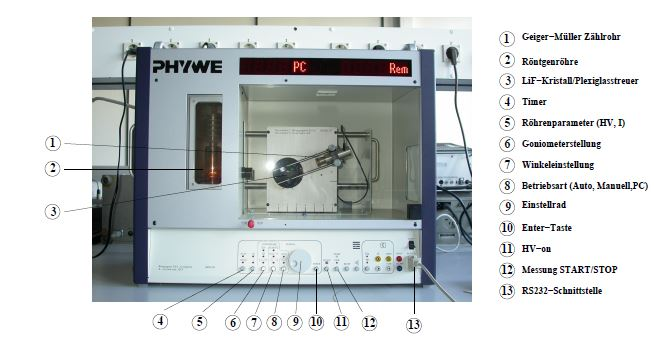
\includegraphics[width=\linewidth]{Bilder/kasten.jpg}
    \caption{Aufbau einer Röntgenröhre \cite{V603}}
    \label{fig:1}
\end{figure}
Die Steuerung der einzelnen Elemente kann Wahlweise per Hand oder Computer erfolgen, jedoch ist es sinnvoll die unterschiedlichen Spektren mit dem Computer aufzunehmen. Die Beschleunigungsspannung
und der Emissionsstrom werden bei allen Messungen auf $U = \SI{35}{\kilo\volt}$ und $I = \SI{1}{\milli\ampere}$ eingestellt.

\subsection{Aufnahme eines Emissionsspektrums der Kupfer Röntgenröhre}
Für die Aufnahme des Emissionsspektrums wird mit dem LiF-Kristall in $\SI{0.1}{\degree}$-Schritten mit einer Integrationszeit von $\SI{10}{\second}$ im Intervall von 
$\SI{8}{\degree}$ bis $\SI{25}{\degree}$ durch gemessen. 

\subsection{Bestimmung der Transmission als Funktion der Wellenlänge}
Für die Bestimmung der Transmission als Funktion der Wellenlänge wird ebenfalls in $\SI{0.1}{\degree}$-Schritten der Kristall abgefahren. Jedoch einmal mit Aluminium-Absorber und einmal ohne.
Bei der Messung mit dem Absorber wird dieser vor die verbaute 2mm Blende gesetzt. Bei beiden Messungen beträgt die Integrationszeit pro Winkel $\SI{200}{\second}$, in einem Winkelbereich von 
$\SI{7}{\degree}$ bis $\SI{10}{\degree}$.

\subsection{Bestimmung der Compton-Wellenlänge }
Für die Bestimmung der Compton-Wellenlänge $\lambda_C$ wird die Transmission der ungestreuten und gestreuten Röntgenstrahlung betrachtet und mit einerander verglichen. Dafür werden die Impulse 
wieder einmal mit und einmal ohne Al-Absorber zwischen Streuer und Geiger-Müller Zählrohr mit einer Integrationszeit von $\SI{300}{\second}$ gemessen.


\section{Vorbereitung}
\label{sub:emilit}
Als Vorbereitung zu dem Versuch sollte die Energien der Cu-$K_\alpha$ und Cu-$K_\beta$ Linie bestimmt und die dazugehörige Wellenlänge $\lambda$ und den Winkel $\alpha$ für den
LiF-Kristall mit der Gitterkonstante $d = \SI{201.4}{\pico\meter}$ und $n = 1$.

\noindent
Die Energien liegen bei $E_{K_\alpha} = \SI{8.046}{\kilo\eV}$ und $E_{K_\beta} = \SI{8.904}{\kilo\eV}$. Daraus folgt für den
Glanzwinkel  $\theta_{K_\alpha} = \SI{22.49}{\degree}$ und $\theta_{K_\beta} = \SI{20.22}{\degree}$ und eine Wellenlänge von $\lambda_{K_\alpha} = \SI{1,54 1e-10}{\meter}$
und $\lambda_{K_\beta} = \SI{1,39 1e-10}{\meter}$.

\noindent
Zusätzlich lässt sich die Compton-Wellenlänge bestimmen zu $\lambda_{K_\text{Compton}} = \SI{2,43 1e-12}{\meter}$.





